\chapter{RESULTS}
\label{ch:evaluation}
The completed results chapter will return to the question posed in the introduction: does guidance spoken in a synthetic version of the participant's own voice differ, in efficiency or experience, from guidance spoken in the neutral voice the participant selected? The chapter will first establish that the intended comparison was delivered, then report search efficiency, and finally examine workload, motivation, and exploratory measures of voice experience. Because no confirmatory participant outcomes are available in this draft, the sections below describe how each result will be reported and distinguish those pending results from the engineering evidence that currently supports the apparatus.

\section{Recorded Development Results}
\label{sec:development-results}
The following descriptive results come from actual headset recordings, rather than simulated trials. The analysis includes all nine locally mirrored \texttt{DEV\_NEUTRAL} recordings dated October 19--20, 2026 (Runs 20--28), with 27 started searches and 21 recorded correct selections. These sessions used the neutral-male development mode; the eight available trial summaries identify the Eric voice and a 168-object layout. This is an earlier development configuration, not the frozen participant-study stimulus configuration. Each recording identifies a different build, and the shared development label does not establish a sample of independent participants. The results therefore describe operation during testing, not a self-similar versus neutral voice effect or a controlled comparison between software versions.

The analysis retains unfinished searches and uses the complete recorded prefix of Run 21, whose final JSON record is truncated. No missing endpoint is reconstructed. Source file hashes, recording identifiers, derived CSV tables, and the plotting script accompany the thesis sources under \texttt{development-results/}. Twenty of the 21 completed-search durations also match the separately saved trial summaries within their 0.01-second rounding precision; Run 21 has no corresponding summary in the inspected mirror. This comparison checks agreement between exports, not independent timing accuracy.

\subsection{Search Completion During Development}
Figure~\ref{fig:development-search} separates completed-search durations from recording coverage. Panel~(a) shows each completed search, with box plots for runs containing at least three completions; runs with fewer completions show individual observations only. Runs with no recorded completion remain labeled with zero observations. Panel~(b) includes all 27 started searches and identifies the six unfinished searches. These unfinished endpoints are not completion times or evidence of task failure: a recording may end while the user is testing, pausing, or leaving the application. The logarithmic duration axis retains the longest completed search while allowing shorter searches to remain distinguishable.

The figures use compact, labeled panels and distribution summaries, following the presentation of descriptive results in Chiossi et al.~\cite{chiossi2024searching}. Boxes span the first and third quartiles, the central line marks the median, and whiskers extend to the most extreme observations within 1.5 interquartile ranges. Every observation remains visible as a point, including values beyond the whiskers. Horizontal offsets separate points for legibility and do not alter measured values. Colors distinguish adjacent runs for readability and do not represent experimental voice conditions. No confidence intervals or significance annotations are estimated from these development recordings.

Among the 21 completed searches, the median recorded active-search duration is 19.56~s, the 95th percentile is 44.43~s, and the maximum is 275.92~s. Percentiles use linear interpolation between ordered observations. The long completed search is retained rather than removed as an outlier: these were unconstrained development sessions, and the logs do not establish that every active second represents uninterrupted task-directed effort. The plotted counter excludes time according to the application's search-timer logic and should not be confused with elapsed recording time. The distribution establishes that the application records completed selections and variable search durations; it does not estimate participant efficiency under a standardized protocol.

\begin{figure}[htbp]
\centering
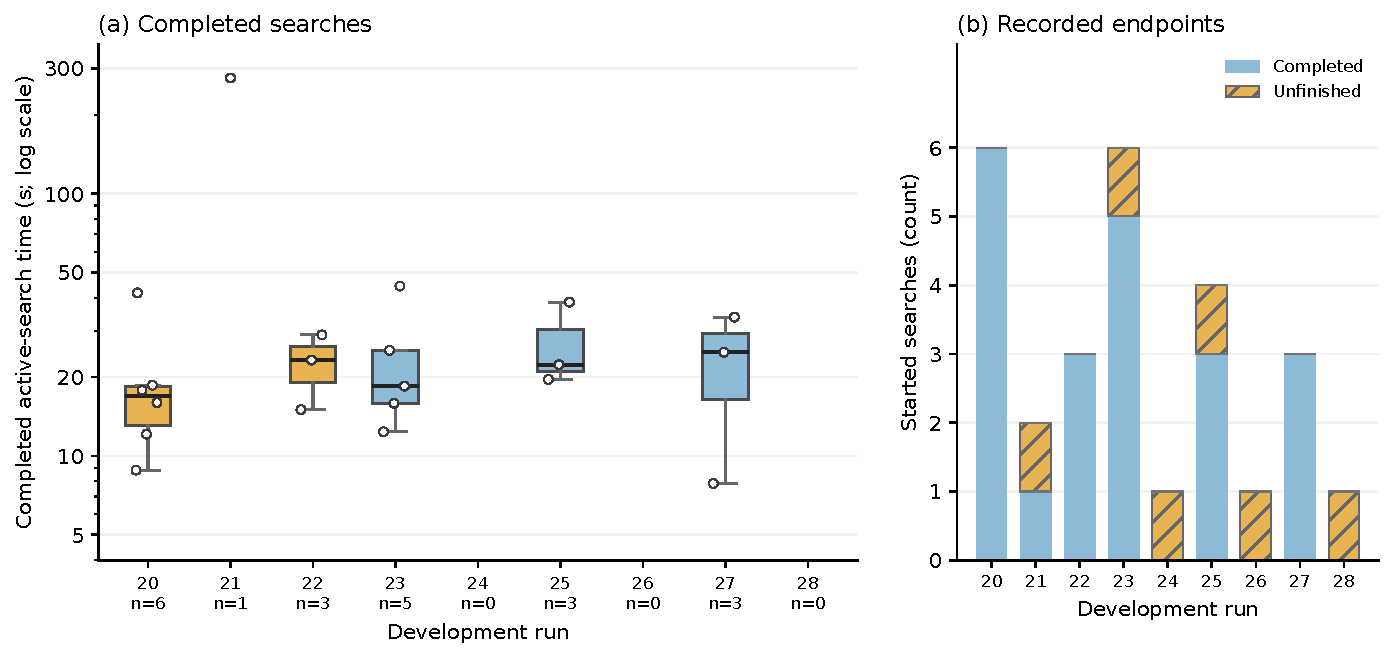
\includegraphics[width=\linewidth,alt={Two panels show development Runs 20 through 28: 21 completed search durations as individual points and quartile boxes on a logarithmic seconds axis, and counts of 21 completed and six unfinished searches. Runs without completions are labeled n equals zero.}]{figures/development-search-times.pdf}
\caption[Recorded development search durations]{Recorded development searches. (a) Completed active-search times, with individual observations, sample counts, and quartile boxes where at least three observations are available; the vertical axis is logarithmic. (b) Counts of completed and unfinished searches. Unfinished searches are excluded from duration summaries, not assigned a completion time.}
\label{fig:development-search}
\end{figure}

\subsection{Speech Delivery and Earlier Waiting}
Of 350 software playback-start events during the recorded search intervals, 339 have an unambiguous chronological match to a guidance request, audio request, and audio-ready event using the same recording, trial, and decision identifier. The remaining 11 playback events are excluded from the latency distribution because the required join is missing or ambiguous. They are not assigned zero delay. Requests that never produced playback also do not enter this delivered-event distribution.

For the 339 matched events, the median interval from the delivered decision's request to software playback is 0.244~s, with a 95th percentile of 0.487~s and a maximum of 0.538~s (Figure~\ref{fig:development-speech}). The median request-to-audio-request interval is 215.7~ms, compared with 17.9~ms from audio request to readiness and 1.0~ms from readiness to playback. The first interval can include decision-making and scheduling; it is not an isolated measurement of Jev network latency. These timestamps measure software events, not the onset of audible sound at the headset.

\begin{figure}[htbp]
\centering
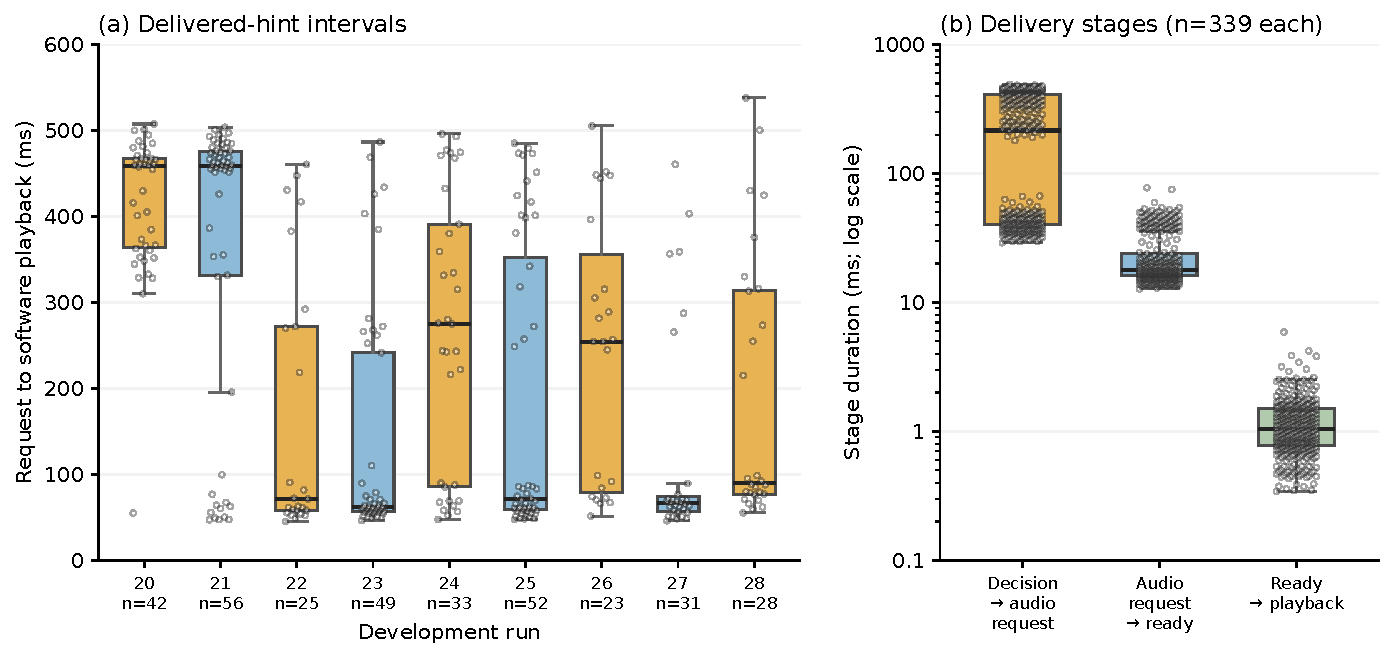
\includegraphics[width=\linewidth,alt={Two panels show 339 matched delivered hints: request-to-playback distributions by development run on a linear milliseconds axis, and the three recorded delivery-stage distributions on a logarithmic milliseconds axis. Each panel shows individual recorded events and quartile boxes.}]{figures/development-speech-delivery.pdf}
\caption[Software speech-delivery intervals]{Software speech-delivery intervals for 339 matched playback events. (a) Request-to-playback distributions by run, with sample counts. (b) Delivery-stage distributions for the same events, using a logarithmic vertical axis. Points retain all observations; boxes and whiskers follow Figure~\ref{fig:development-search}. Earlier qualification and deferral, undelivered requests, and acoustic onset are outside this measure.}
\label{fig:development-speech}
\end{figure}

Short delivery intervals do not establish prompt feedback from the user's perspective. Figure~\ref{fig:development-confirmation} reconstructs the previously investigated gaze-confirmation episode in Run 20, Trial 4. A gaze-qualified hint request is recorded at session time 321.426~s. Three successive transmission snapshots record qualified target gaze, while controller-hold qualification is false. Jev returns \emph{wait}, \emph{wait}, and then \emph{speak}; playback of ``You've got it!'' begins at 323.616~s. The interval from the first qualified request to playback is therefore 2.190~s, although the final request-to-playback interval is only about 0.352~s. This is one delayed episode with repeated requests, not three independent confirmation failures. The snapshots document qualification at those instants; they do not independently establish uninterrupted fixation between them.

\begin{figure}[htbp]
\centering
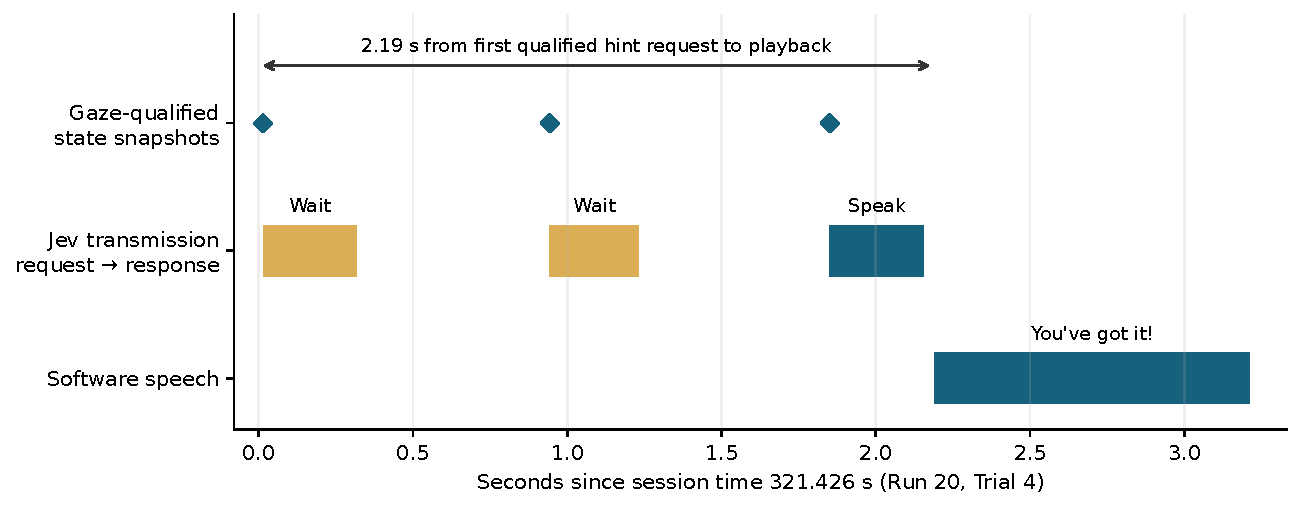
\includegraphics[width=\linewidth,alt={Run 20 Trial 4 timeline: three gaze-qualified snapshots accompany two wait decisions and a speak decision. The confirmation begins 2.19 seconds after the first qualified request. Controller hold is unqualified at all three snapshots.}]{figures/development-confirmation-sequence.pdf}
\caption[Recorded gaze-confirmation delay]{Recorded gaze-confirmation delay in Run 20, Trial 4. Diamonds mark qualified-state snapshots, bars mark transmission request/response intervals and software speech. Gaze confirmation is distinct from controller confirmation and correct trigger selection.}
\label{fig:development-confirmation}
\end{figure}

This case demonstrates why sequence history is required alongside aggregate delivery statistics. Earlier waiting remains visible even when the request that ultimately produces speech is processed quickly. The historical recording does not establish whether subsequent changes eliminated this behavior; that question requires a comparable recording from the revised build. No acoustic-latency or participant-perception conclusion is drawn from this trace.

\subsection{Recorded Gaze Usability}
Figure~\ref{fig:development-gaze} summarizes 58,041 rendered-frame replay samples recorded during active search. A sample is counted as usable when the saved gaze-device availability flag is true and the replay's gaze-usable flag is set. This is the application's recorded usability decision, which includes tracking and freshness checks, rather than a new physiological classification. Samples marked unusable are retained, and absent or indeterminate flags would be classified as unknown.

Across the nine runs, usable-row fractions range from 63.75\% to 99.97\%. All inspected active-search rows have a usable/unusable classification; however, intervals with no recorded rows remain unobserved and are not included in the denominator. The dominant logged invalidity reason is \texttt{both\_native\_eyes\_invalid}. That diagnostic does not by itself distinguish blinking, headset removal, poor fit, calibration, or a software issue. Runs with long periods of unusable gaze warrant timeline inspection before they are used to assess guidance behavior.

\begin{figure}[htbp]
\centering
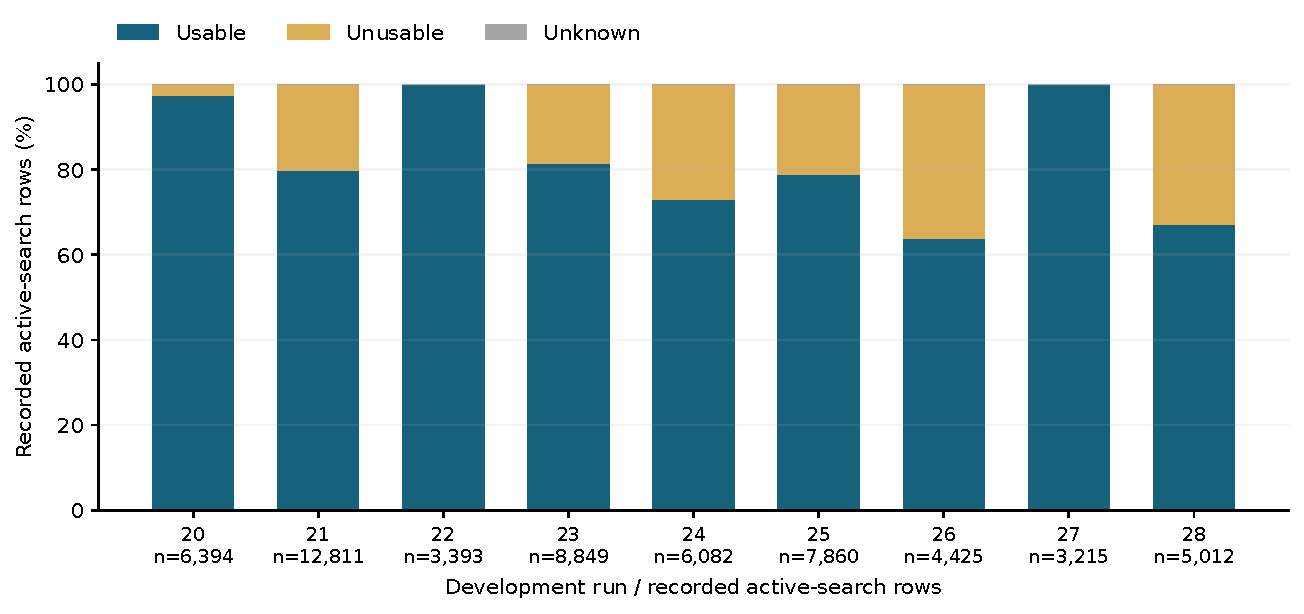
\includegraphics[width=\linewidth,alt={Stacked bars show usable and unusable active-search replay rows for development Runs 20 through 28, with denominators below each bar. Usable fractions range from 63.75 to 99.97 percent; no inspected row has an unknown flag.}]{figures/development-gaze-usability.pdf}
\caption[Recorded gaze usability during development]{Recorded gaze usability during active search, with the number of replay rows shown for each run. These are rendered-frame observations, not independent native sensor samples. Unrecorded intervals are outside the denominator.}
\label{fig:development-gaze}
\end{figure}

The row fractions are not estimates of spatial accuracy, native acquisition frequency, fixation quality, or the proportion of total search time with valid gaze. Their role is diagnostic: they identify differences in the evidence available to the guidance system during these development recordings. Together, the search, delivery, and usability plots document the apparatus before the planned voice comparison, while leaving performance and experience differences between voices unresolved.

\subsection{Exploratory Eye-Measurement Pipeline}
\label{sec:development-eye-candidates}
A separate analysis uses the recorded eye-observation file for development Run 30 (October 23, 2026), which contains five recorded search identifiers in neutral-male mode. These searches precede the new deadline configuration; their retained durations are not truncated to 25 seconds. Figure~\ref{fig:development-eye-candidates} presents per-eye candidate fixation counts, candidate saccade rates, exploratory IPA, and pupil duration retained for IPA. The figure uses only measured records; artificial test signals used to verify the code are excluded.

The strict pupil screens retain approximately 2.18, 2.25, 4.22, and 5.28 seconds per eye for the first four searches, with no accepted segment for the fifth. These short retained windows are not estimates of whole-trial workload, and an unavailable IPA value is not a zero. Separate left- and right-eye values expose disagreement rather than averaging it away. The candidate fixation counts and restricted saccade rates likewise depend on detection thresholds and on the available query-time evidence. Three illustrative parameter variants are exported for sensitivity inspection, without choosing a setting on the basis of a favorable result.

\begin{figure}[htbp]
\centering
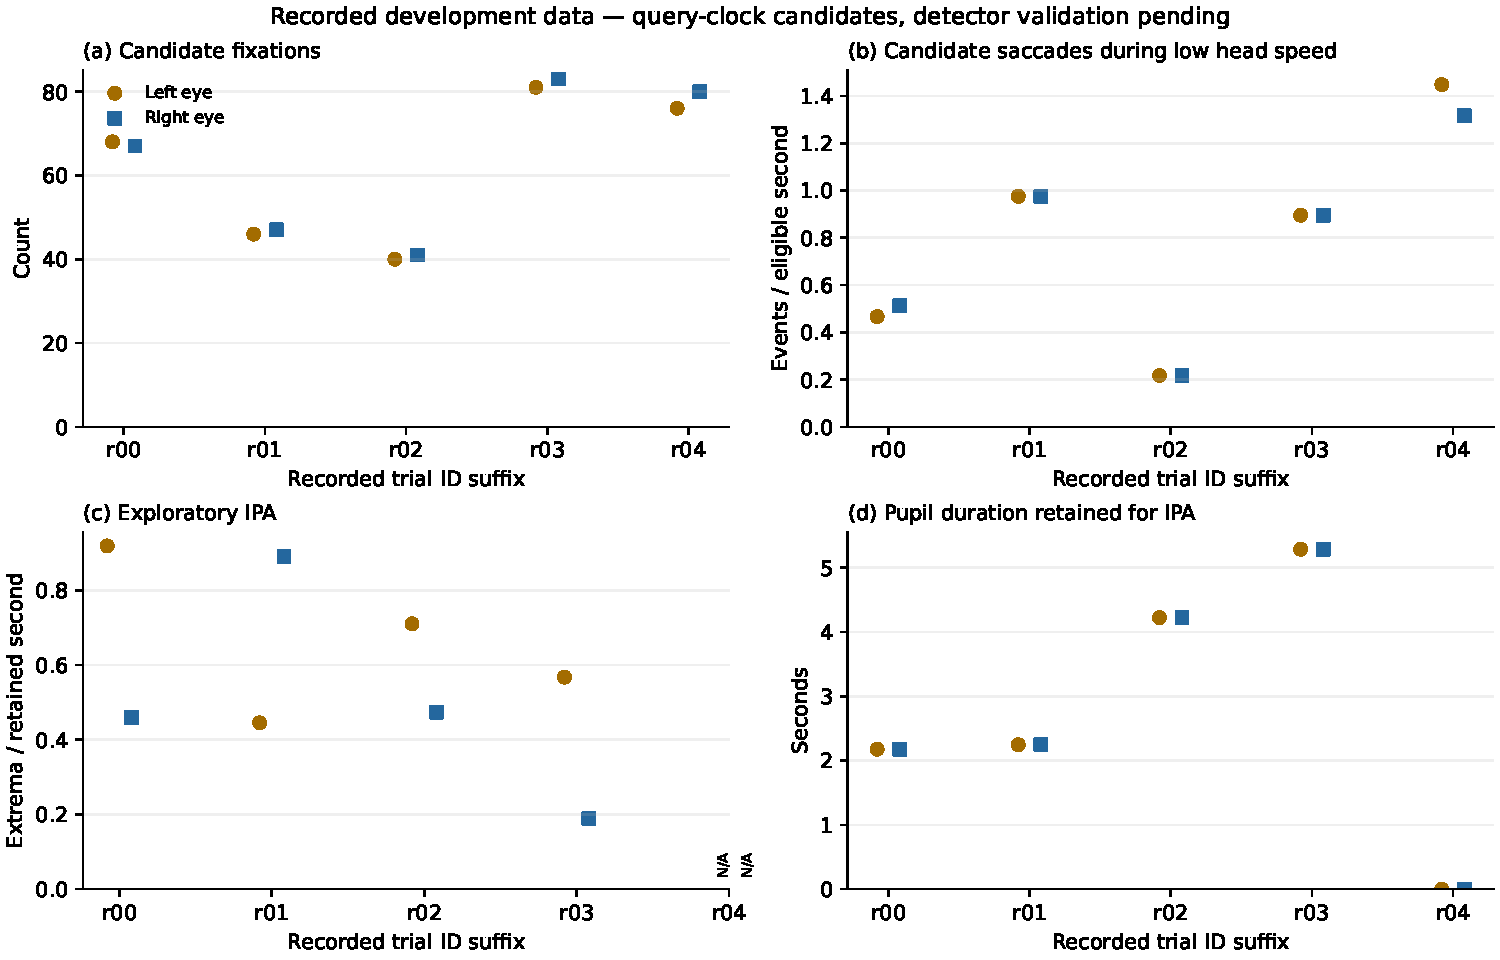
\includegraphics[width=\linewidth,alt={Four panels show actual Run 30 per-eye candidate fixation counts, saccade rates during low head speed, exploratory IPA and retained pupil duration for five searches. The fifth search has unavailable IPA. All eye-event classifications remain unvalidated.}]{figures/development-eye-candidates.pdf}
\caption[Exploratory eye-measurement output from recorded data]{Run 30 development diagnostics. (a) Candidate fixation counts. (b) Candidate saccade events per retained low-head-speed second. (c) Exploratory IPA extrema per retained pupil second. (d) Retained pupil duration. Points represent separate eyes within recorded searches, not independent participants. The software-query clock does not establish 120-Hz sensor acquisition, and the classifications require independent validation.}
\label{fig:development-eye-candidates}
\end{figure}

The source hash, detector configuration, dependency versions, individual event intervals, summary CSV, and threshold-sensitivity table are retained with the thesis development artifacts. Computational checks pass, but no independently labeled headset sequence is yet available to establish event precision, recall, or duration error. These results demonstrate an executable measurement workflow and identify data limitations; they do not supply participant-study findings.

\subsection{Outcome Panels by Voice Condition}
\label{sec:development-voice-panels}
Figure~\ref{fig:development-voice-panels} adapts the four-panel presentation of accuracy, missed targets, search time, and pupil activity in Chiossi et al.~\cite{chiossi2024searching} to the present study's voice conditions. Each horizontal axis distinguishes \emph{Neutral voice} from \emph{Self-similar voice}; AR/VR and physical/virtual subdivisions are not factors in this comparison. The current observations come from development Run 30. Its five started searches all use the neutral voice, so the self-similar position remains explicitly unpopulated. Scheduled searches that never started do not contribute observations.

First-selection accuracy is 80\%: four of the five completed searches contain no incorrect trigger selection before the correct selection. This is a run-level proportion among completed searches, rather than a distribution across participants or a measure of success before the new deadline. Active-search completion times use the recorded search counter and retain their original values in seconds. Run 30 has no recorded 25-second deadline, so its missed-target percentage is unavailable; searches lasting longer than 25 seconds are not retrospectively classified as misses.

For the condition-level display, exploratory IPA is the arithmetic mean of the available left- and right-eye candidate rates within each search. Four searches have values from both eyes; the fifth has no eligible pupil segment and remains missing. This display summary is not a validated workload score, and the separate-eye diagnostics and retained durations remain available in Figure~\ref{fig:development-eye-candidates}. Points in the time and IPA panels denote repeated trials within one development run. They do not represent independent participants, and the figure supports no estimate of a voice-condition effect. The participant-study comparison requires observations from both voices and paired participant summaries using consistent scoring and eligibility rules.

\begin{figure}[htbp]
\centering
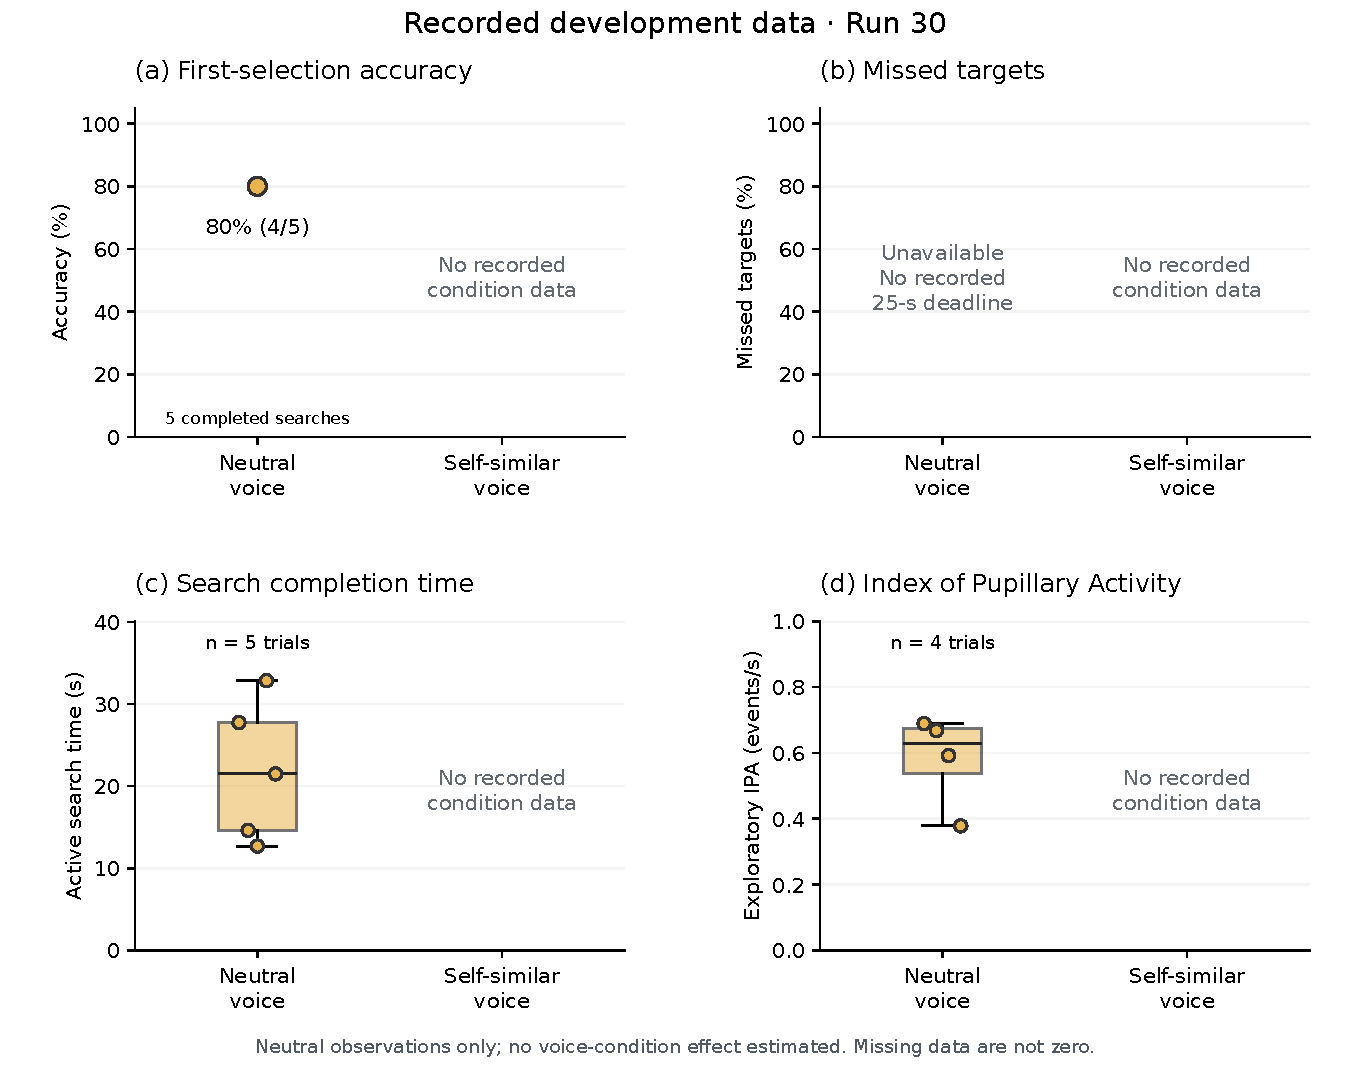
\includegraphics[width=\linewidth,alt={Four development outcome panels use Neutral voice and Self-similar voice on every horizontal axis. Neutral Run 30 has 80 percent first-selection accuracy among five completed searches, five active search times, and four exploratory IPA trial means. Missed-target percentage is unavailable without a recorded deadline. Self-similar data are absent in every panel.}]{figures/development-voice-condition-panels.pdf}
\caption[Development outcome panels by voice condition]{Development outcome panels arranged for the neutral versus self-similar voice comparison. (a) First-selection accuracy among completed searches, shown as one run-level point. (b) Missed targets, unavailable for this recording without a recorded deadline. (c) Active search completion time. (d) Exploratory IPA averaged across available eyes within each trial. Boxes in (c) and (d) show quartiles and median, with 1.5-IQR whiskers; all observed trial values are shown. Unavailable values are not plotted as zero. No self-similar observations or inferential comparisons are included.}
\label{fig:development-voice-panels}
\end{figure}


\section{Planned Reporting of Participant Results}
The completed empirical chapter will first report participant flow, exclusions, incomplete sessions, and data coverage by condition and order. It will then describe realized starting geometry and the similarity manipulation check before presenting the primary voice contrast. This order allows readers to assess whether the intended comparison was delivered and measured.

The primary result will include the fitted time contrast, its uncertainty, the analyzed participant and trial counts, and model diagnostics. Secondary sections will then report workload and IMI subscales at participant-by-block level, followed by exploratory sections on agent perception, voice experience, guidance behavior, and debrief themes. Each table will state its denominator and identify missing observations, so that changes in the analyzed sample remain visible.

\begin{table}[htbp]
\centering\caption{Planned result families and their current status. No confirmatory participant outcomes are reported in this draft.}
\small\tagpdfsetup{table/header-rows={1}}
\begin{tabularx}{\linewidth}{@{}p{0.27\linewidth}XX@{}}\toprule
Result family & Required evidence & Present status \\\midrule
Participant flow & Consented, started, completed, stopped; reasons & Not available \\
Manipulation check & Similarity by voice with paired scope & Not available \\
Primary performance & Adjusted time contrast and uncertainty & Not estimated \\
Workload and IMI & Versioned raw items and complete subscales & Not collected for this report \\
Agent experience & Individual and construct-specific ratings & Not collected for this report \\
Guidance quality & Sequence-level playback and evidence & Development traces reported; study comparison pending \\
Debrief themes & Recorded responses and coding audit & Not available \\\bottomrule
\end{tabularx}
\end{table}


\subsection{Results Organized by Research Question}
Following the manipulation check, each research question will be answered in turn. For RQ1, the estimate will be the marginal time contrast standardized over a common starting-difficulty distribution, as defined in Section~\ref{ch:analysis}; here, \emph{standardized} refers to that common distribution rather than to a standardized effect size. The estimate will be accompanied by its uncertainty, the eligible participant and trial counts, and model diagnostics, following the analysis plan finalized before confirmatory recruitment. RQ2 will report the paired workload outcomes and the separate IMI subscales, using multiplicity families that the analysis plan has yet to fix. RQ3 will present exploratory agent-perception and custom ratings alongside debrief themes and valid search measures. A contrast that cannot be estimated or proves inconclusive will be reported as such rather than omitted.

EQ1 will be reported separately through sequence coverage, qualification-to-playback delay, provider reliability, and categorized faults. These engineering measures assess the delivery of guidance, while the participant study evaluates differences between voices. As summarized in Table~\ref{tab:rq-map}, neither a passing software test nor a favorable model rating establishes an effect on participants; likewise, a voice-condition difference does not verify that every instruction was delivered correctly.

\section{User Performance}
Participant-study estimates are not yet available; this section is reserved for active search-completion time, incorrect trigger selections, and valid gaze/controller contact latencies by voice condition. Reporting will include paired participant summaries and the planned adjusted contrast, with sample counts and uncertainty. Recorded development runs may illustrate delivery or export behavior in a separately labeled pilot analysis, but cannot establish that one voice improves participant performance.

\section{User Experience}
Participant ratings are not yet available; this section is reserved for condition-referenced workload, the separate motivation subscales, agent experience, voice liking and similarity, and debrief responses. Results will retain the distinction between preference, perceived resemblance, and task performance. No questionnaire response or preference distribution is generated from synthetic trials.

\section{Evidence Available for This Draft}
Alongside the recorded development results in Section~\ref{sec:development-results}, engineering verification records document the apparatus. These sources do not constitute confirmatory participant-study outcomes. The October 20 alignment audit documents software checks, analysis tests, and a successful Android build, installation, and launch. These records support specific implementation claims; they do not bear on a treatment effect, perceived naturalness, eye-tracker accuracy, or acoustic response latency.

The audit reports passing schedule and voice-isolation checks, including one practice trial in the first assigned voice, two measured blocks, and nominal-angle quotas, and it records 38 trial-export tests and seven workload scoring/plot tests. These counts describe the audit's own test run, not a suite re-executed for this manuscript, so any later claim based on them should cite the verification record and the revision it tested.

\begin{table}[htbp]
\centering\caption{Evidence status at the documented implementation checkpoint.}
\small\tagpdfsetup{table/header-rows={1}}
\begin{tabularx}{\linewidth}{@{}p{0.28\linewidth}XX@{}}\toprule
Evidence & Supported conclusion & Boundary \\\midrule
Schedule and voice checks & One practice and nominal 40-by-two allocation pass fixtures & Does not verify wearer completion of a full session \\
Trial export and TLX tests & Declared scales and retrospective joins pass tested cases & Not validation of all questionnaires \\
Unity integration checks & Listed state and interaction fixtures pass & Not proof against all timing races \\
Android build/install/launch & Application built, installed, and started & Not a participant acceptance session \\
Exact pre-cue theta & Required definition documented & Snapshot implementation remains a gap \\
Vertical allocation & Cross-relative definition documented & 20/20 enforcement remains a gap \\
Voice-condition outcomes & No confirmatory dataset reported & No performance or preference conclusion \\\bottomrule
\end{tabularx}
\end{table}


\section{Guidance Quality Supporting the Voice Contrast}
The completed report will describe gaze availability, actual speech exposure, delayed acknowledgments, interruptions, and unhelpful cues by voice condition and session. This account will help assess whether technical delivery problems affected one condition more than the other. The voice contrast will not automatically be adjusted for behavior-dependent hint counts or waiting time: these quantities arise after voice assignment, may themselves depend on voice condition, and cannot be treated as baseline difficulty (Section~\ref{ch:analysis}).

Gaze acknowledgment, controller acknowledgment, and correct trigger selection remain separate events. Their sequence records document feedback delivery, whereas participant ratings and debriefing address how that feedback was experienced. Advisory model judgments cannot substitute for those participant reports. Appendix~\ref{app:guidance-support} describes the policy pilots, episode definitions, failure categories, and investigation of two-second delays that support assessment of the apparatus before interpreting differences between voices.
